\documentclass[12pt]{article}

\usepackage{fontawesome}
\usepackage{hyperref}
\usepackage{xurl}
\usepackage{graphicx}
\usepackage{float}
\usepackage[tagged, highstructure]{accessibility}
\usepackage{bookmark}
\usepackage{enumitem}

\hypersetup{
    colorlinks=false,
    pdfborder={0 0 0},
    pdftitle={Breach Analysis Lab},
    pdfauthor={Adrianna Holden-Gouveia},
    pdfsubject={Information Security - Lab Assignment},
    pdflang={en-US},
    pdfkeywords={data breach, breach notice, FTC, Massachusetts 93H, Have I Been Pwned}
}

% Configure PDF bookmarks for navigation
\bookmarksetup{
    numbered,
    open,
}

% Configure list spacing for better accessibility
\setlist{nosep}



\title{Breach Analysis}
\author{
        Adrianna Holden-Gouveia \\
        Website: \href{https://aholdengouveia.name}{aholdengouveia.name}\\ 
        \date{\vspace{-5ex}}
        %Email: \href{mailto:admin@aholdengouveia.name}{admin@aholdengouveia.name} \\
%        \faLinkedin{: aholdengouveia} \\
        \faGithub {: aholdengouveia} \\
        \faTwitter {: aholdengouveia} \\
        }

%S\date{\today}


\begin{document}    

\maketitle

\section*{Accessibility Notice}
This document is also available in HTML format at:

Link: \href{https://aholdengouveia.name/InfoSec/labs/breachanalysis.html}{\textbf{\nolinkurl{https://aholdengouveia.name/InfoSec/labs/breachanalysis.html}}}

The HTML version provides enhanced accessibility features including keyboard navigation, screen reader support, responsive design, dark mode support, and high contrast options.


%\begin{abstract}
%This is a template for Linux Administration Lab work
%\end{abstract}
%\tableofcontents

\section*{Learning Outcomes}
By the end of this lab, you will be able to:
\begin{itemize}
    \item Find a recent data breach, and the notice the company sent to the people affected
    \item Compare a company's breach response with the FTC's best practices and Massachusetts law
    \item Explain how combining stolen data with other data can cause more harm, and whether a breach was an insider or outsider threat
    \item Check whether your own data has been in a breach, and take steps to protect yourself
\end{itemize}

\section*{Lab Instructions}
When a company has a data breach, it's supposed to tell the people affected. In this lab, you'll find a real breach notice, check it against best practices, follow how the company handled it, and then check your own data.

\subsection*{Screenshots}
This lab asks for at least 8 screenshots. Each screenshot should have your name, term, and year.  One of the easiest ways to do that is make a text document with your name and term/year on your computer and save it to use all term. Any screenshots that don't include this information won't be counted.

\begin{figure}[H]
    \centerline{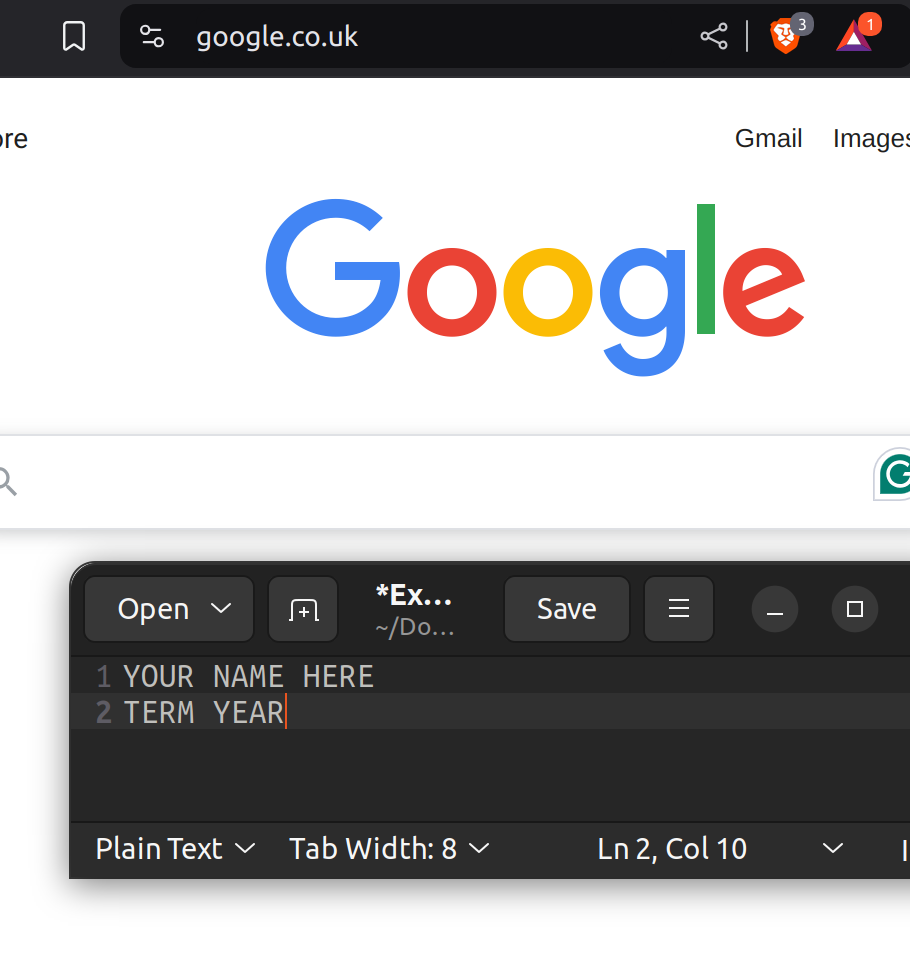
\includegraphics[scale=.2]{ExampleScreenshot.png}}
    \caption{This is an image of what each of your screenshots should look like}
    \alt{Example screenshot: a web browser showing the Google home page, with a small text editor window in front of it that says YOUR NAME HERE and TERM YEAR}
\end{figure}

You can blur or cover anything private in a screenshot, such as your email address, as long as your name and term note still shows.

\subsection*{Part 1: Find a Breach and Its Notice}
Pick a data breach from the last 2 years. It can be from anywhere, but you need to be able to find the notice the company sent to the people affected. Good places to look:
\begin{itemize}
    \item Massachusetts posts the breach notice letters companies send to residents, sorted by month (linked under Resources)
    \item The company's own website, often on a page called ``notice of data security incident''
    \item News articles, which often link to the notice
\end{itemize}
Breaches from class, such as PowerSchool (2024) and Canvas (2026), are fine to use.
\begin{enumerate}
    \item Give the company's name, when the breach happened, and a link to the notice.
    \item Take a screenshot of the notice, showing the company's name and the date.
\end{enumerate}

\subsection*{Part 2: Build a Timeline}
Find at least 4 dated events, each from a different kind of source:
\begin{itemize}
    \item The notice itself
    \item A news article
    \item A statement from the company, such as a press release, a blog post, or a post on its social media
    \item One more, such as a social media post from someone affected, a state filing, or a second news article
\end{itemize}
For each event, include the date, what happened, a citation, and a screenshot of the source showing its title and date.
\begin{enumerate}[start=3]
    \item Put the events in order. When did the breach start? When did the company find it? When did people find out?
    \item How long did people wait between the company finding the breach and being told? Was that reasonable? Why or why not?
    \item Did the company's story match what the news reported? Point out anything that was different.
\end{enumerate}
For the news articles, also include a CRAAP check. My guide to evaluating sources, linked under Resources, shows how.

\subsection*{Part 3: Score the Notice}
The FTC's Data Breach Response guide lists what a good notice should include. Massachusetts law, Chapter 93H, adds its own rules. Both are linked under Resources.
\begin{enumerate}[start=6]
    \item Make a table with three columns: the item, your score (Met, Partly met, or Not met), and your evidence. For evidence, quote the exact words from the notice, or write ``not in the notice''. Score these items:
    \begin{enumerate}
        \item Says what information was taken
        \item Says what the company has done to fix the problem
        \item Tells you what you can do to protect yourself
        \item Offers help, such as free credit monitoring or identity protection
        \item Gives a way to contact the company, such as a phone number or website
        \item Was sent quickly. Use your timeline.
        \item Is written so someone without a tech background could understand it
        \item Says how the breach happened. \textbf{Massachusetts letters aren't allowed to include this}, so if yours is a Massachusetts letter, write ``not allowed in Massachusetts'', and find out how it happened from the news instead.
        \item Tells you that you have the right to get a police report (Massachusetts law)
        \item Explains how to freeze your credit, and that a credit freeze is free (Massachusetts law)
    \end{enumerate}
    If your breach isn't from Massachusetts, still score the last two. Would the notice have met Massachusetts law?
    \item Overall, how well did the company do? Give 2 things it should have done better, and support each one with the FTC guide or an expert source.
\end{enumerate}

\subsection*{Part 4: Connect the Dots}
\begin{enumerate}[start=8]
    \item List every type of data the notice says was taken, such as names, email addresses, Social Security numbers, or medical information.
    \item Pick one other place an attacker could get information about the same people, such as another breach, social media, or a people-search website. What could an attacker learn by combining the two? Give one specific way they could use it to cause harm.
    \item Was this breach an insider threat, from someone inside the company, or an outsider threat, from someone outside? Remember, insider threats include mistakes, not just people doing harm on purpose. If it's not known, say what you think and why.
    \item Would you still trust this company with your data? Why or why not?
\end{enumerate}

\subsection*{Part 5: Check Your Own Data}
Have I Been Pwned is a free website that checks whether an email address has been in a known data breach. Use an email address you use, or a family member's with their permission. You can blur the address in your screenshot.
\begin{enumerate}[start=12]
    \item Search the address, and take a screenshot of the results.
    \item If it was in a breach, pick one. What data was taken? If it wasn't in any breaches, pick a breach from the site's list of recent breaches, and answer for that one.
    \item Take 2 steps to protect yourself, and take a screenshot of each. For example: change the password for that account, turn on two-factor authentication, or find the page that explains how to freeze your credit at Equifax, Experian, or TransUnion. You don't have to actually freeze your credit.
    \item Which of your 2 steps would help most if your data from Part 4 was combined with other data? Why?
\end{enumerate}

\section*{Deliverables}
One file that includes:
\begin{itemize}
    \item Part 1: your breach, the link, and your screenshot of the notice
    \item Part 2: your timeline of at least 4 events, each with a citation and screenshot, CRAAP checks for the news articles, and your answers
    \item Part 3: your scoring table, and your answer
    \item Part 4: your answers
    \item Part 5: your 3 screenshots, and your answers
\end{itemize}

\section*{Resources}
References, a video, a PowerPoint and some notes are available at my website
Link: \href{https://www.aholdengouveia.name/InfoSec/PolicyCompliance.html}{\textbf{\nolinkurl{https://www.aholdengouveia.name/InfoSec/PolicyCompliance.html}}}

FTC: Data Breach Response, A Guide for Business, for Part 3
Link: \href{https://www.ftc.gov/business-guidance/resources/data-breach-response-guide-business}{\textbf{\nolinkurl{https://www.ftc.gov/business-guidance/resources/data-breach-response-guide-business}}}

Massachusetts General Laws Chapter 93H, Section 3: what a breach notice to residents must and must not include, for Part 3
Link: \href{https://malegislature.gov/Laws/GeneralLaws/PartI/TitleXV/Chapter93H/Section3}{\textbf{\nolinkurl{https://malegislature.gov/Laws/GeneralLaws/PartI/TitleXV/Chapter93H/Section3}}}

Massachusetts data breach notification reports and letters, for Part 1
Link: \href{https://www.mass.gov/lists/data-breach-notification-reports}{\textbf{\nolinkurl{https://www.mass.gov/lists/data-breach-notification-reports}}}

Have I Been Pwned, for Part 5
Link: \href{https://haveibeenpwned.com/}{\textbf{\nolinkurl{https://haveibeenpwned.com/}}}

FTC: Credit Freezes and Fraud Alerts, for Part 5
Link: \href{https://consumer.ftc.gov/articles/what-know-about-credit-freezes-and-fraud-alerts}{\textbf{\nolinkurl{https://consumer.ftc.gov/articles/what-know-about-credit-freezes-and-fraud-alerts}}}

My guide to evaluating sources
Link: \href{https://www.aholdengouveia.name/Howtos/Sourceeval/sourceEvaluation.html}{\textbf{\nolinkurl{https://www.aholdengouveia.name/Howtos/Sourceeval/sourceEvaluation.html}}}

The CRAAP test, with questions to ask about each source
Link: \href{https://web.archive.org/web/20250814000638/https://guides.lib.uchicago.edu/c.php?g=1241077&p=9082343}{\textbf{\nolinkurl{https://web.archive.org/web/20250814000638/https://guides.lib.uchicago.edu/c.php?g=1241077&p=9082343}}}

\end{document}
